% MACE methodology; \input after the Introduction.
% Preamble dependencies: \usepackage{graphicx,booktabs,array,amsmath,amssymb,tikz}
% \usetikzlibrary{arrows.meta,positioning,calc,fit,matrix}
% Figure paths assume compilation from repository root. See docs/paper/MACE_Methodology_Figures_README.md.
\section{Methodology}
\label{sec:methods}

\subsection{Control-driven dynamics and forecasting task}
\label{sec:methods:problem}

We consider a dynamical system whose physical state $\mathbf{x}(t)$ evolves under a prescribed control trajectory $\mathbf{u}(t)$, with fixed physical and numerical parameters $\boldsymbol{\eta}$. The reference simulator defines
\begin{equation}
  \dot{\mathbf{x}}(t)=\mathbf{f}\!\left(\mathbf{x}(t),\mathbf{u}(t);\boldsymbol{\eta}\right),
  \qquad
  \mathbf{y}(t)=\mathbf{g}\!\left(\mathbf{x}(t),\mathbf{u}(t);\boldsymbol{\eta}\right),
  \label{eq:mace:system}
\end{equation}
where $\mathbf{y}(t)\in\mathbb{R}^{J}$ denotes the selected \emph{output variables}, rather than necessarily a vector of independently integrated state quantities. A \emph{control trajectory} specifies the actuator history. Its simulation produces a \emph{multivariate response trajectory}; the paired control and response, together with initialization and sampling metadata, form a \emph{trajectory sample}. A \emph{forecast trajectory} is the ordered sequence of surrogate predictions obtained from an initial output history and the known future control, without subsequently revealing the simulator response.

For trajectory sample $i$, let $h=0,\ldots,H-1$ index a common fixed-origin forecast grid, $j=1,\ldots,J$ index output variables, and $m=1,\ldots,M$ index ensemble members. In the present application the control is the common angle $\theta(t)$ imposed on twelve drums, $J=15$, $M=10$, and $t_h=0.4h$~s, so $H=501$ covers 0--200~s. A horizon is a position in this grid, not an independently initialized forecast with new observations at each $h$. The reference response is used as the accuracy and interval-coverage target, not as a correction signal during rollout.

Table~\ref{tab:mace:notation} establishes the distinction between data and uncertainty terms. We use \emph{calibration distribution} for the population supplying conformal scores and \emph{evaluation distribution} for the population on which accuracy, coverage, and width are assessed. Whether their trajectory samples are exchangeable determines the scope of the ordinary split-conformal argument.

\begin{table}[t]
\centering\small
\caption{Forecasting and calibration terminology. All simultaneous coverage events refer to the recorded forecast grid.}
\label{tab:mace:notation}
\begin{tabular}{@{}p{0.31\linewidth}p{0.63\linewidth}@{}}
\toprule
Term & Definition\\
\midrule
Control trajectory & Prescribed time history $\mathbf{u}(t)$ (here drum angle $\theta(t)$).\\
Multivariate response trajectory & Simulator outputs $\{\mathbf{y}(t_h)\}_{h=0}^{H-1}$.\\
Trajectory sample & Control and associated simulator response, with initial-condition metadata.\\
Forecast trajectory & Recursively predicted outputs $\{\widehat{\mathbf y}(t_h)\}_h$.\\
Calibration distribution & Distribution providing held-out trajectory-level scores.\\
Evaluation distribution & Distribution of trajectory samples on which intervals are tested.\\
MACE-Horizon & Separate conformal threshold for each $(h,j)$.\\
MACE-Trajectory & Separate threshold for each $j$ after maximizing its score over $h$.\\
Horizon complete multivariate coverage & All $J$ outputs covered at a specified $h$.\\
Trajectory complete multivariate coverage & All $J$ outputs covered at every evaluated $h$.\\
\bottomrule
\end{tabular}
\end{table}

\subsection{Stochastic control-trajectory sampling}
\label{sec:methods:sampling}

Sampling independent actuator positions at successive time steps would produce inputs whose instantaneous amplitudes may be admissible but whose temporal variation is not representative of sustained physical excitation. Instead, we prescribe a covariance for \emph{control velocity} and integrate its realizations to obtain continuous, piecewise-linear angle trajectories. This construction makes the correlation time, accumulated angular dispersion, and initial control condition independently interpretable. It is prespecified sampling, not uncertainty-directed acquisition of additional simulations.

On a uniform control grid $t_r=r\Delta_c$, $\Delta_c=0.1$~s and $r=0,\ldots,L$, with $L=2000$, let $\mathbf{v}=(v_0,\ldots,v_{L-1})^{\mathsf T}$ contain interval velocities in degrees per second. Before conditioning the initial velocity, the implemented Mat\'ern-$5/2$ covariance is
\begin{equation}
 K_{rs}=s_v\left(1+a_{rs}+\frac{a_{rs}^{2}}{3}\right)e^{-a_{rs}}
 +(n_v+\varepsilon_v)\delta_{rs},
 \qquad a_{rs}=\frac{\sqrt{5}\lvert t_r-t_s\rvert}{\ell},
 \label{eq:mace:velocitycov}
\end{equation}
where $s_v$ is the velocity sill in $(^\circ/\mathrm{s})^2$, $\ell$ is the correlation length, $n_v$ is the nugget, and $\varepsilon_v=(s_v+n_v)\varepsilon_{\mathrm{frac}}$ is numerical covariance jitter. Omitting nugget and jitter, the stationary velocity semivariogram is $\gamma_v(\Delta)=s_v[1-\rho_v(\Delta)]$, with $\rho_v$ the parenthesized Mat\'ern correlation. This is a semivariogram for the velocity process; the integrated angle process is generally nonstationary.

Defining $B_{kr}=\Delta_c$ when $r<k$ and zero otherwise, the left-endpoint integration is
\begin{equation}
  \boldsymbol{\theta}=\theta_0\mathbf{1}+B\mathbf{v},
  \qquad
  \operatorname{Cov}(\boldsymbol{\theta})=BKB^{\mathsf T}.
  \label{eq:mace:integratedcontrol}
\end{equation}
The generator initializes $\theta_0=45^\circ$ and conditions the first interval velocity to zero. Specifically, an unconditioned draw is transformed by subtracting $K_{:0}v_0/(K_{00}+\varepsilon_c)$ and then setting its first component exactly to zero; $\varepsilon_c$ regularizes the conditioning denominator. The angle table is subsequently formed by integration. The control signal consumed by Modelica is an interpolation of that tabulated angle, rather than a continuously differentiable analytic Gaussian-process realization.

The velocity sill is selected using an \emph{unconditioned} endpoint-dispersion design. For correlation $\rho_v$, define
\begin{equation}
 A(\ell)=L+2\sum_{r=1}^{L-1}(L-r)\rho_v(r\Delta_c),\qquad
 s_v=\frac{\sigma_{\theta,\mathrm{design}}^2/\Delta_c^2-n_vL}{A(\ell)}.
 \label{eq:mace:sill}
\end{equation}
For the documented batch-3 configuration, $\ell=10$~s, $\sigma_{\theta,\mathrm{design}}=2.5^\circ$, $n_v=0$, $\varepsilon_{\mathrm{frac}}=10^{-10}$, $\varepsilon_c=10^{-10}$, and the random seed is 123. The endpoint design standard deviation is not the standard deviation after conditioning and rejection. For exact reproduction, the covariance of the implemented regularized linear transformation, with the first velocity fixed at zero, must be propagated through $B$ rather than equating it to the unconditioned design covariance.

Generated profiles are rejected if any angular position falls outside $0^\circ$--$180^\circ$. The original stochastic trajectories selected for this study were specified to share the velocity semivariogram and to satisfy $|\dot{\theta}|<1^\circ/\mathrm{s}$; this retained-sample rate condition should not be confused with a rate rejection performed by the current covariance generator, which checks angle bounds but does not itself implement a hard velocity threshold. The generation manifests and saved velocity tables are the required evidence for verifying the full original population and its realized rate extrema. Figure~\ref{fig:mace:sampling} illustrates the Mat\'ern correlation, sample velocities and angles, and the distinct unconditioned and initialized dispersion curves.

\begin{figure*}[t]
\centering
\includegraphics[width=\textwidth]{outputs/paper/mace_figures/sampling/fig01_control_trajectory_sampling.pdf}
\caption{Construction of stochastic control trajectories from Mat\'ern-$5/2$ interval velocities. (a) Analytic velocity correlations for alternative correlation lengths, highlighting the retained $\ell=10$~s design. (b,c) Paired velocity and integrated-angle realizations on the 0.1-s control grid, initialized at $45^\circ$; the figure metadata distinguish actual batch-3 profiles from illustrative draws. (d) Unconditioned design and regularized zero-initial-velocity angle dispersion before bounded-path rejection. The $2.5^\circ$ terminal value is a design target, not a hard angle bound or the conditioned endpoint.}
\label{fig:mace:sampling}
\end{figure*}

Each accepted control trajectory is applied to the same reference simulation under the prescribed initial operating condition. Simulator responses are stored on the coarser, common 0.4-s output grid. The selected original partitions contain 5,000 training, 1,000 validation, 1,000 calibration, and 2,000 evaluation trajectory samples. The split is by whole trajectory, so time windows from a single sample do not cross partitions. Independence additionally requires verifying that shared-parent branches or duplicate controls did not enter different partitions; the current study does not use branching as a sampling or acquisition method.

\subsection{LSTM ensemble training and autoregressive forecasting}
\label{sec:methods:forecasting}

A recurrent surrogate maps a finite history of output variables and a shifted window of known controls to the next multivariate response. Let $\boldsymbol{\xi}$ denote neural-network input features, explicitly distinct from the physical state $\mathbf{x}(t)$. The training-only min--max transformations use native input coordinates $X$ and output coordinates $Y$,
\begin{equation}
 \widetilde{\xi}^{X}_{a}=\frac{\xi_a-a_a^X}{b_a^X},
 \qquad
 \widetilde y^{Y}_{j}=\frac{y_j-a_j^Y}{b_j^Y},
 \label{eq:mace:scaling}
\end{equation}
where $a$ is the appropriate training minimum, $b$ is the training range (replaced with unity for a constant feature), and the superscript identifies the fitted coordinate system. The same stored scaler is used for every forecast, calibration, and evaluation distribution; extrapolating scaled values are not clipped or refitted.

For the configured lookback $K=12$, the sequence builder includes both history endpoints. To predict output $\mathbf y_{k+1}$, row $r=0,\ldots,K$ contains the pair
\begin{equation}
 \left[\widetilde{\mathbf y}^{\,X}_{k-K+r},
       \widetilde{\mathbf u}^{\,X}_{k-K+1+r}\right].
 \label{eq:mace:window}
\end{equation}
Consequently the input has $13$ rows and $16$ features, consisting of the history of 15 output variables over $k-12,\ldots,k$ and the one prescribed drum angle over $k-11,\ldots,k+1$. Prepared steady-state rows initialize the first forecast at time zero. This indexing ensures the control corresponding to the predicted output time is available without supplying its unobserved response.

The ensemble contains ten LSTM predictors with identical architecture but independently sampled training subsets. Each member is trained on a 70\% subset of the 5,000 training trajectories, drawn without replacement within that member; subsets may overlap between members. This is subsampling-based ensemble training, not conventional with-replacement bootstrapping. The network comprises one LSTM layer with 64 hidden units, the final recurrent output, a $64\!\to\!64$ linear layer, a rectified linear activation, and a $64\!\to\!15$ output layer. Models optimize one-step mean-squared error using Adam, train with batch size 64 over at most 100 epochs, and restore the lowest-validation-loss checkpoint. The learning rate begins at $3\times10^{-4}$ and is halved after each 30 epochs; the configured early-stopping patience of 1,000 does not ordinarily stop a 100-epoch run. Configuration values and profile counts are summarized in Table~\ref{tab:mace:training}.

\begin{table}[t]
\centering\small
\caption{Stored stochastic-dataset and ensemble training configuration.}
\label{tab:mace:training}
\begin{tabular}{@{}p{0.50\linewidth}p{0.44\linewidth}@{}}
\toprule
Quantity & Setting\\
\midrule
Training / validation / calibration / evaluation & 5,000 / 1,000 / 1,000 / 2,000 trajectories\\
Forecast horizon / output grid & 501 points; 0--200 s; 0.4 s\\
Inputs / outputs & $13\times16$ / 15\\
Ensemble size / member sample & 10 / 70\% training trajectories\\
Architecture & LSTM(64), Linear(64,64), ReLU, Linear(64,15)\\
Optimizer / objective & Adam / one-step MSE\\
Epochs / batch / learning rate & 100 / 64 / $3\times10^{-4}$\\
Learning-rate schedule & StepLR(30, 0.5)\\
Scaler / validation selection & Training-only min--max / best validation checkpoint\\
\bottomrule
\end{tabular}
\end{table}

For evaluation, every member is initialized from the same prepared history and recursively uses \emph{its own} preceding predictions. Importantly, a predicted vector in output-scaled coordinates cannot generally be inserted directly into the history expressed in input-scaled coordinates. For output variable $j$, feedback therefore uses
\begin{equation}
 \widehat{\widetilde y}^{\,X}_{m,h,j}
 =\widehat{\widetilde y}^{\,Y}_{m,h,j}\frac{b_j^Y}{b_j^X}
 +\frac{a_j^Y-a_j^X}{b_j^X}.
 \label{eq:mace:feedback}
\end{equation}
The mapped vector is cast at the neural-network input boundary, the oldest history row is dropped, and the prescribed control window advances. Reference outputs are withheld after initialization. Neither the ensemble mean nor another member's predictions are used for member feedback. This correct native-coordinate recurrence is used in the operational evaluation; archival stochastic results generated using direct $Y$-to-$X$ feedback require an equivalent corrected rerun before their numerical values can be compared on the same basis.

In output-scaled coordinates the frozen ensemble produces
\begin{equation}
 \mu_{i,h,j}=\frac{1}{M}\sum_{m=1}^{M}\widehat{\widetilde y}^{\,Y}_{m,i,h,j},
 \qquad
 \sigma_{i,h,j}=\left[\frac{1}{M}\sum_{m=1}^{M}
 \bigl(\widehat{\widetilde y}^{\,Y}_{m,i,h,j}-\mu_{i,h,j}\bigr)^2\right]^{1/2}.
 \label{eq:mace:ensemble}
\end{equation}
The population convention ($\mathrm{ddof}=0$) is used. Here $\sigma$ measures member disagreement, not the standard error of the ensemble mean, and does not by itself define a calibrated Gaussian predictive distribution. The physical-unit ensemble mean is recovered using the saved output scaler. Figure~\ref{fig:mace:lstm} distinguishes one-step network architecture from member-specific recursive inference.

\begin{figure*}[t]
\centering
% Requires tikz libraries arrows.meta,positioning,calc,fit.
\resizebox{\textwidth}{!}{%
\begin{tikzpicture}[>=Latex, font=\sffamily\small,
  unit/.style={draw=black!70,rounded corners=2pt,fill=blue!4,inner sep=5pt,align=center},
  prog/.style={-{Latex[length=2.5mm]},line width=.85pt,draw=blue!70!black},
  ctrl/.style={-{Latex[length=2.3mm]},dashed,draw=black!80,line width=.65pt}]
 \node[anchor=west,font=\bfseries] at (0,4.1) {(a) Network for one ensemble member};
 \node[unit,minimum width=2.8cm,minimum height=1.15cm] (x) at (1.65,2.9) {History and control\\$B_{\rm batch}\times13\times16$};
 \node[unit,minimum width=2.05cm,minimum height=1.15cm] (l) at (4.55,2.9) {LSTM\\one layer, 64 units};
 \node[unit,minimum width=1.55cm] (last) at (6.86,2.9) {Last row\\$B_{\rm batch}\times64$};
 \node[unit,minimum width=2.05cm] (fc) at (9.35,2.9) {Linear $64\to64$\\ReLU};
 \node[unit,minimum width=1.6cm] (pred) at (11.83,2.9) {Linear $64\to15$};
 \draw[prog] (x)--(l); \draw[prog] (l)--(last); \draw[prog] (last)--(fc); \draw[prog] (fc)--(pred);
 \node[align=center,font=\scriptsize] at (1.65,1.86) {15 output-history features\\$+\,1$ prescribed control};
 \node[anchor=west,font=\bfseries] at (0,1.15) {(b) Autoregression; member-specific feedback};
 \node[unit,minimum width=2.4cm] (hist) at (1.5,.18) {History in $X$\\13 rows $\times$ 15};
 \node[unit,minimum width=2.35cm] (fm) at (4.7,.18) {$f_m$ with shifted\\prescribed control};
 \node[unit,minimum width=2.2cm] (yh) at (8.02,.18) {$\widehat{\widetilde{\mathbf y}}^{Y}_{m,h}$\\15 output values};
 \node[unit,minimum width=2.15cm] (map) at (11.36,.18) {$Y\to X$ affine map\\then shift history};
 \draw[prog] (hist)--(fm); \draw[prog] (fm)--(yh); \draw[prog] (yh)--(map);
 \draw[prog,rounded corners=6pt] (map.south)--++(0,-.75)-|(hist.south);
 \node[font=\scriptsize,fill=white,inner sep=1pt] at (6.4,-.77) {Next horizon: member $m$ feeds back its own mapped prediction};
 \node[unit,minimum width=2.35cm] (u) at (4.72,-1.75) {Known control\\$u_{k-K+1:k+1}$};
 \draw[ctrl] (u.north)--(fm.south);
 \node[unit,minimum width=2.55cm] (agg) at (11.15,-1.75) {After all $M=10$ members\\mean $\mu_h$, spread $\sigma_h$};
 \draw[prog] (yh.south east) to[out=-37,in=100] (agg.north);
 \draw[densely dotted,black!45] (-.1,1.62)--(13.2,1.62);
 \node[font=\scriptsize,anchor=west,text=black!70] at (.05,-2.65) {Blue solid: forecast or recurrence \hspace{9mm} Black dashed: prescribed controls \hspace{9mm} No future simulator-response feedback};
\end{tikzpicture}%
}

\caption{Autoregressive LSTM ensemble. (a) Implemented $13\times16$ input window, one 64-unit recurrent layer, and 15-output prediction head. (b) Each member receives known shifted controls, predicts in output coordinates, converts that prediction into input coordinates, and updates its own history. Ten independently trained members are aggregated only after individual forecasts; no future reference responses or ensemble-mean feedback enter a member's recurrence.}
\label{fig:mace:lstm}
\end{figure*}

\subsection{MACE: ensemble-normalized conformal prediction}
\label{sec:methods:mace}

MACE uses the ensemble mean for interval centering and its time- and output-dependent spread for adaptive interval scaling. With a single positive additive floor $\tau=10^{-3}$ in output-scaled units, define
\begin{equation}
 d_{i,h,j}=\sigma_{i,h,j}+\tau,\qquad
 s_{i,h,j}=\frac{\left|\widetilde y^{\,Y}_{i,h,j}-\mu_{i,h,j}\right|}{d_{i,h,j}}.
 \label{eq:mace:score}
\end{equation}
The floor keeps the nonconformity score defined when ensemble members agree closely; it is common across outputs and horizons. Forecast-dependent adaptation arises only through $d$. The scale is not a trained conditional variance and the calibration step does not update network parameters. For outputs with persistently small spread, such as steam quality in some operating conditions, the floor may dominate, reducing variation in interval width. A larger floor need not monotonically widen the final interval because its conformal multiplier changes.

All calibrations use independent \emph{whole trajectory samples} as statistical units. For a nonconformity-score sample $R_1,\ldots,R_{N_{\mathrm{cal}}}$, the split-conformal threshold is the $k$-th smallest score without interpolation, where $k=\lceil(N_{\mathrm{cal}}+1)(1-\alpha)\rceil$. With $N_{\mathrm{cal}}=1{,}000$ and $\alpha=0.05$, $k=951$. The finite-threshold implementation requires $k\leq N_{\mathrm{cal}}$; the usual theoretical infinite-threshold convention when $k>N_{\mathrm{cal}}$ does not arise here.

We use three score reductions and corresponding calibrated events. First, \emph{MACE-Horizon} retains $s_{i,h,j}$ and calculates a separate $q_{h,j}$ across calibration samples for every horizon--output pair. The interval $I_{h,j}=[\mu_{h,j}\!-\!q_{h,j}d_{h,j},\mu_{h,j}\!+\!q_{h,j}d_{h,j}]$ targets marginal coverage of a specified $(h,j)$; the quantiles form an $H\times J$ array. Second, \emph{MACE-Trajectory} reduces each calibration trajectory to $R_{i,j}=\max_h s_{i,h,j}$ and selects one threshold $q_j$ per output variable. It targets the event that the entire \emph{single-output} forecast trajectory stays inside its band on the evaluated grid. Third, for \emph{joint trajectory calibration}, each sample contributes one scalar $R_i=\max_{h,j}s_{i,h,j}$ before selecting $q_{\mathrm{all}}$. The resulting common threshold targets every output variable at every evaluated horizon simultaneously, namely Trajectory complete multivariate coverage. Taking the maximum of independently calibrated $q_j$ is not equivalent to this scalar-score calibration.

These objectives must not be conflated with empirical complete multivariate diagnostics. \emph{Horizon complete multivariate coverage} requires every output to be contained in its interval at a fixed horizon, whereas \emph{Trajectory complete multivariate coverage} requires containment for all $(h,j)$ in the evaluated grid. MACE-Horizon does not directly calibrate the former event; that would require a horizon-level joint score such as $\max_j s_{i,h,j}$, which is not among the evaluated calibrations. Similarly, MACE-Trajectory's per-output trajectory guarantee does not imply complete multivariate trajectory coverage. Figure~\ref{fig:mace:events} depicts the distinct score reductions and events, with the illustrative event grids deliberately smaller than the actual $501\times15$ forecast.

\begin{figure*}[t]
\centering
% Editable conceptual figure, requiring tikz/arrows.meta/calc/positioning.
\resizebox{\textwidth}{!}{%
\begin{tikzpicture}[>=Latex,font=\sffamily\small, box/.style={draw=black!75,rounded corners=2pt,fill=blue!3,align=center,minimum height=.67cm,inner sep=4pt},
arr/.style={-{Latex[length=2.4mm]},line width=.8pt,draw=black!70}]
 \node[anchor=west,font=\bfseries] at (-.1,6.90) {(a) Frozen forecast and calibration score};
 \node[box,minimum width=2.9cm] (ens) at (1.45,6.2) {Frozen ten-member\\forecast trajectories};
 \node[box,minimum width=2.55cm] (stats) at (5.15,6.2) {Mean $\mu$ and\\population spread $\sigma$};
 \node[box,minimum width=2.4cm] (d) at (8.65,6.2) {Positive scale\\$d=\sigma+\tau$};
 \node[box,minimum width=2.35cm] (s) at (12.1,6.2) {Normalized error\\$s=|\widetilde y-\mu|/d$};
 \node[box,minimum width=2.3cm] (truth) at (12.1,5.20) {Held-out calibration\\response $\widetilde y$};
 \draw[arr] (ens)--(stats); \draw[arr] (stats)--(d); \draw[arr] (d)--(s);
 \draw[arr] (truth.north)--(s.south);
 \node[font=\bfseries,anchor=west] at (-.1,4.65) {(b) Per-trajectory score reduction and coverage event};
 \node[font=\scriptsize,anchor=west] at (0,4.18) {Construction};
 \node[font=\scriptsize,anchor=west] at (3.4,4.18) {Within each calibration trajectory};
 \node[font=\scriptsize,anchor=west] at (7.4,4.18) {Across $N_{\mathrm{cal}}=1000$ trajectories};
 \node[font=\scriptsize,anchor=west] at (11.9,4.18) {Event on 5$\times$3 schematic grid};
 \foreach \YY/\NAME/\REDUCE/\QQ/\HIGHLIGHT in {
  3.30/{MACE-Horizon}/{retain $(h,j)$}/{$q_{h,j}$}/1,
  2.18/{MACE-Trajectory}/{$\max_h s_{i,h,j}$}/{$q_j$}/2,
  1.06/{Joint trajectory}/{$\max_{h,j}s_{i,h,j}$}/{$q_{\mathrm{all}}$}/3
 } {
   \node[box,minimum width=2.8cm] at (1.55,\YY) {\NAME};
   \node[box,minimum width=2.7cm] at (5.1,\YY) {\REDUCE};
   \node[box,minimum width=2.1cm] at (9.05,\YY) {$k=951$th\\\QQ};
   \draw[arr] (2.95,\YY)--(3.73,\YY);
   \draw[arr] (6.53,\YY)--(7.92,\YY);
   \draw[arr] (10.15,\YY)--(11.0,\YY);
   \foreach \j in {0,1,2}{
    \foreach \h in {0,1,2,3,4}{
      \pgfmathtruncatemacro{\FILL}{(\HIGHLIGHT==3)||(\HIGHLIGHT==2 && \j==1)||(\HIGHLIGHT==1 && \h==2 && \j==1)}
      \ifnum\FILL=1
        \fill[blue!24] (11.45+.36*\h,\YY-.29+.19*\j) rectangle ++(.36,.19);
      \fi
      \draw[black!65,line width=.3pt] (11.45+.36*\h,\YY-.29+.19*\j) rectangle ++(.36,.19);
    }
   }
 }
 \node[align=left,font=\scriptsize,anchor=west] at (13.52,3.30) {One horizon--output\\pair};
 \node[align=left,font=\scriptsize,anchor=west] at (13.52,2.18) {One output over\\all horizons};
 \node[align=left,font=\scriptsize,anchor=west] at (13.52,1.06) {Every output at\\every horizon};
 \draw[black!60,densely dashed] (0,.37)--(16,.37);
 \draw[blue!60!black,line width=.85pt] (1.35,-.12) rectangle ++(.38,.49);
 \node[font=\scriptsize,anchor=west,align=left] at (1.95,.10) {Horizon complete multivariate event: one entire column (all outputs at fixed $h$).};
 \node[font=\scriptsize,anchor=west,align=left] at (1.95,-.19) {Diagnostic under ordinary MACE-Horizon; not a fourth calibrated construction.};
 \node[box,minimum width=7.0cm] at (8.0,-1.02) {Shared interval: $\quad I_{h,j}=[\mu_{h,j}-q\,(\sigma_{h,j}+\tau),\;\mu_{h,j}+q\,(\sigma_{h,j}+\tau)]$};
\end{tikzpicture}%
}

\caption{MACE score construction and conformal coverage objectives. (a) The frozen ensemble supplies mean and spread; held-out calibration responses yield normalized scores. (b) Separate order statistics across trajectory samples are formed from individual $(h,j)$ scores, each output's maximum over time, or each sample's maximum over time and outputs. Highlighted $5\times3$ grids schematically indicate the event targeted by each construction; they are not empirical success maps. Horizon complete multivariate coverage remains a diagnostic for MACE-Horizon, not an additional calibrated procedure.}
\label{fig:mace:events}
\end{figure*}

Conditional on the frozen ensemble, scaler, floor and score reduction, exchangeability of calibration and evaluation \emph{trajectory samples} makes the corresponding scalar scores exchangeable. The conformal order statistic then provides finite-sample marginal coverage for the chosen event. Dependence across horizons or outputs \emph{within} a sample does not invalidate this trajectory-level construction. Its finite-sample statement is population-marginal, applies to the recorded grid, and does not guarantee a fixed coverage rate within every control family, phase, or individual trajectory. Training trajectories can come from a different distribution without invalidating the split-calibration argument, provided the calibrated predictor remains fixed and the calibration/evaluation samples satisfy the required exchangeability. Changing the evaluation distribution without recalibration generally removes that ordinary guarantee.

To separate the value of spread-based scaling from calibration itself, we construct matched \emph{absolute-error conformal} baselines by replacing $s_{i,h,j}$ with $\lvert\widetilde y^{\,Y}_{i,h,j}-\mu_{i,h,j}\rvert$. The same reductions, calibration sets, conformal rank, and coverage events are retained, while $d$ is replaced by one for interval construction. Any displayed $\mu\pm2\sigma$ envelope is only an uncalibrated ensemble diagnostic. This matched comparison avoids mistaking the simultaneous-coverage effect of taking a maximum for an efficiency improvement due to adaptive scaling.

\subsection{Reduced microreactor simulator and transient responses}
\label{sec:methods:plant}

The demonstration system is a reduced Modelica model executed with Dymola, coupling a six-delayed-group point-kinetics representation to lumped reactor and balance-of-plant heat transfer. The plant model resolves twelve synchronized control drums through a common angle but does not resolve three-dimensional neutronics, spatial heat-pipe fields, or a deployed controller. Reactor power is $P=P_r n$ with $P_r=6$~MW; $n$ is normalized power. The physical state contains $n$, six precursor quantities $c_r$, and five thermal nodes $T_f,T_m,T_{hp},T_{N2},T_{sg}$, for twelve differential states. Reactivity, calculated steam outlet temperature, and calculated steam quality are additional algebraic output variables. In the present model,
\begin{equation}
 \dot n=\frac{\rho-\beta}{\Lambda}n+\sum_{r=1}^{6}\lambda_r c_r,\qquad
 \dot c_r=\frac{\beta_r}{\Lambda}n-\lambda_r c_r,
 \qquad
 \rho=\rho_{\mathrm{drums}}(\theta)+\alpha_f(T_f-T_{f0})+\alpha_m(T_m-T_{m0}).
 \label{eq:mace:kinetics}
\end{equation}
The drum contribution follows the model's cosine worth relationship referenced to $\theta_0=45^\circ$. Thermal energy balances couple the fuel, moderator/structure, effective heat-pipe, nitrogen-loop, and active steam-generator metal nodes. Figure~\ref{fig:mace:plant} illustrates the modeled pathways and prescribed secondary boundaries.

\begin{figure*}[t]
\centering
% Vector abstraction of the implemented reduced Modelica thermal network.
\resizebox{\textwidth}{!}{%
\begin{tikzpicture}[>=Latex,font=\sffamily\small,
 n/.style={draw=black!75,rounded corners=3pt,fill=blue!4,align=center,minimum width=2.05cm,minimum height=1.02cm,inner sep=4pt},
 a/.style={-{Latex[length=2.5mm]},line width=1pt,draw=blue!65!black},
 f/.style={-{Latex[length=2.1mm]},line width=.7pt,dashed,draw=black!70}]
 \node[font=\bfseries,anchor=west] at (-.1,3.17) {Point kinetics / synchronized reactivity control};
 \node[n,fill=black!3,minimum width=2.4cm] (angle) at (1.3,2.3) {Prescribed drum\\angle $\theta(t)$};
 \node[n,minimum width=3.0cm] (kin) at (5.0,2.3) {Six-group point kinetics\\$n,c_1,\ldots,c_6$};
 \node[n,minimum width=2.4cm] (pf) at (8.55,2.3) {$P=6n$ MW\\power deposition};
 \draw[f] (angle)-- node[above,font=\scriptsize] {12 equal-angle drums} (kin);
 \draw[a] (kin)--(pf);
 \node[n] (fuel) at (1.0,.32) {Fuel\\$T_f$};
 \node[n] (moderator) at (3.75,.32) {Moderator / structure\\$T_m$};
 \node[n] (hp) at (6.5,.32) {Effective heat pipes\\$T_{hp}$};
 \node[n] (n2) at (9.25,.32) {Nitrogen loop\\$T_{N2}$};
 \node[n] (sg) at (12,.32) {Active SG metal\\$T_{sg}$};
 \draw[a] (fuel)--(moderator);
 \draw[a] (moderator)--(hp);
 \draw[a] (hp)--(n2);
 \draw[a] (n2)--(sg);
 \draw[a] (pf.south) to[out=-95,in=90] (moderator.north);
 \draw[a] (pf.south east) to[out=-55,in=90] (fuel.north);
 \draw[f] (fuel.north) to[out=105,in=-105] (kin.south);
 \draw[f] (moderator.north) to[out=105,in=-60] (kin.south);
 \node[align=center,font=\scriptsize] at (5.25,1.18) {Temperature reactivity feedback};
 \node[n,fill=orange!5,minimum width=2.85cm] (fw) at (15.4,.32) {Feedwater / steam\\secondary-side closure};
 \draw[a] (sg)--(fw);
 \node[font=\scriptsize,align=center] at (15.4,-.70) {Prescribed $\dot m_{\rm fw},p_{\rm out}$\\Calculated $T_{\rm steam,out},x_{\rm steam,out}$};
 \node[font=\scriptsize,anchor=west,text=black!70] at (-.05,-1.0) {Thermal nodes denote lumped energy balances; no turbine, full-fluid inventory, or spatial multiphysics is resolved.};
\end{tikzpicture}%
}

\caption{Reduced point-kinetics and heat-transfer network for the offline microreactor demonstration. Twelve synchronized drums supply the prescribed angle $\theta(t)$. Reactor power and thermal feedback couple five thermal nodes. The steam-generator metal node receives heat from the nitrogen node and transfers heat to a feedwater/steam stream with prescribed mass flow and outlet pressure; steam outlet temperature and quality are calculated. Connections represent lumped energy exchange rather than spatially resolved components.}
\label{fig:mace:plant}
\end{figure*}

In particular, the active steam-generator metal is a dynamic thermal capacitance, not a constant-temperature sink or the thermal mass of the full secondary fluid inventory:
\begin{equation}
 \begin{split}
 C_{sg}\dot T_{sg}&=Q_{N2\rightarrow sg}-Q_{sg\rightarrow fw},\\
 Q_{N2\rightarrow sg}&=G_{N2,sg}(T_{N2}-T_{sg}),\\
 Q_{sg\rightarrow fw}&=\max\{G_{sg,fw}(T_{sg}-T_{\mathrm{sat}}),0\}.
 \end{split}
 \label{eq:mace:steammetal}
\end{equation}
The added specific heat $q_{sg}=Q_{sg\rightarrow fw}/\dot m_{\mathrm{fw}}$ determines the simplified saturated-mixture and superheat closures,
\begin{equation}
 x_{\mathrm{steam,out}}=
 \begin{cases}
 0,&q_{sg}\leq0,\\
 q_{sg}/h_{fg},&0<q_{sg}<h_{fg},\\
 1,&q_{sg}\geq h_{fg},
 \end{cases}
 \quad
 T_{\mathrm{steam,out}}=
 \begin{cases}
 T_{\mathrm{sat}},&q_{sg}<h_{fg},\\
 T_{\mathrm{sat}}+(q_{sg}-h_{fg})/c_{p,\mathrm{sh}},&q_{sg}\geq h_{fg}.
 \end{cases}
 \label{eq:mace:steamclosure}
\end{equation}
Here $h_{fg}$ is the specified latent heat and $c_{p,\mathrm{sh}}$ is an effective superheated-steam heat capacity. Thus outlet temperature and quality are \emph{calculated}, not prescribed, despite possible saturation plateaus or quality saturation. The secondary outlet pressure and feedwater flow are fixed at 1.5~MPa and 2.95~kg/s. The active-metal capacitance passed by the executed \texttt{RunOneProfile} wrapper is $2.55\times10^5$~J/K, which supersedes the plant class default when no run-time override is supplied. The simulator reference uses the wrapper's 200-s horizon and $10^{-8}$ tolerance; a specific solver/version is not inferred from these settings.

The 15 stored output variables, in native output order, are $T_{N2}$, $T_m$, $T_{hp}$, $T_f$, $T_{sg}$, $c_1,\ldots,c_6$, $n$, $\rho_{\$}$, $T_{\mathrm{steam,out}}$, and $x_{\mathrm{steam,out}}$. Here $\rho_{\$}=\rho/\beta$ is reactivity in dollars; the normalized precursor quantities retain the simulator's implemented normalization, rather than assumed physical concentration units. Table~\ref{tab:mace:outputs} distinguishes differential outputs from algebraic closures and notes that the displayed dataset uses physical power $P=6n$~MW in place of normalized $n$. The simulator traces in Figure~\ref{fig:mace:dataset} illustrate the training-distribution response variety, not forecast performance.

\begin{table}[t]
\centering\small
\caption{Native forecasting output variables. Power $P$ in the displayed 4$\times$4 dataset figure replaces the stored normalized $n$ only for visualization; drum angle is a prescribed input.}
\label{tab:mace:outputs}
\begin{tabular}{@{}l p{0.44\linewidth} l l@{}}
\toprule
Indices & Quantity / symbol & Units & Type\\
\midrule
1 & Nitrogen-node $T_{N2}$ & K & ODE\\
2 & Moderator/structure $T_m$ & K & ODE\\
3 & Effective heat-pipe $T_{hp}$ & K & ODE\\
4 & Fuel $T_f$ & K & ODE\\
5 & Steam-generator metal $T_{sg}$ & K & ODE\\
6--11 & Delayed precursor $c_1,\ldots,c_6$ & normalized & ODE\\
12 & Neutron population $n$ & -- & ODE\\
13 & Reactivity $\rho_{\$}$ & dollars & algebraic\\
14 & Steam outlet $T_{\mathrm{steam,out}}$ & K & algebraic\\
15 & Steam outlet $x_{\mathrm{steam,out}}$ & -- & algebraic\\
\bottomrule
\end{tabular}
\end{table}

\begin{figure*}[t]
\centering
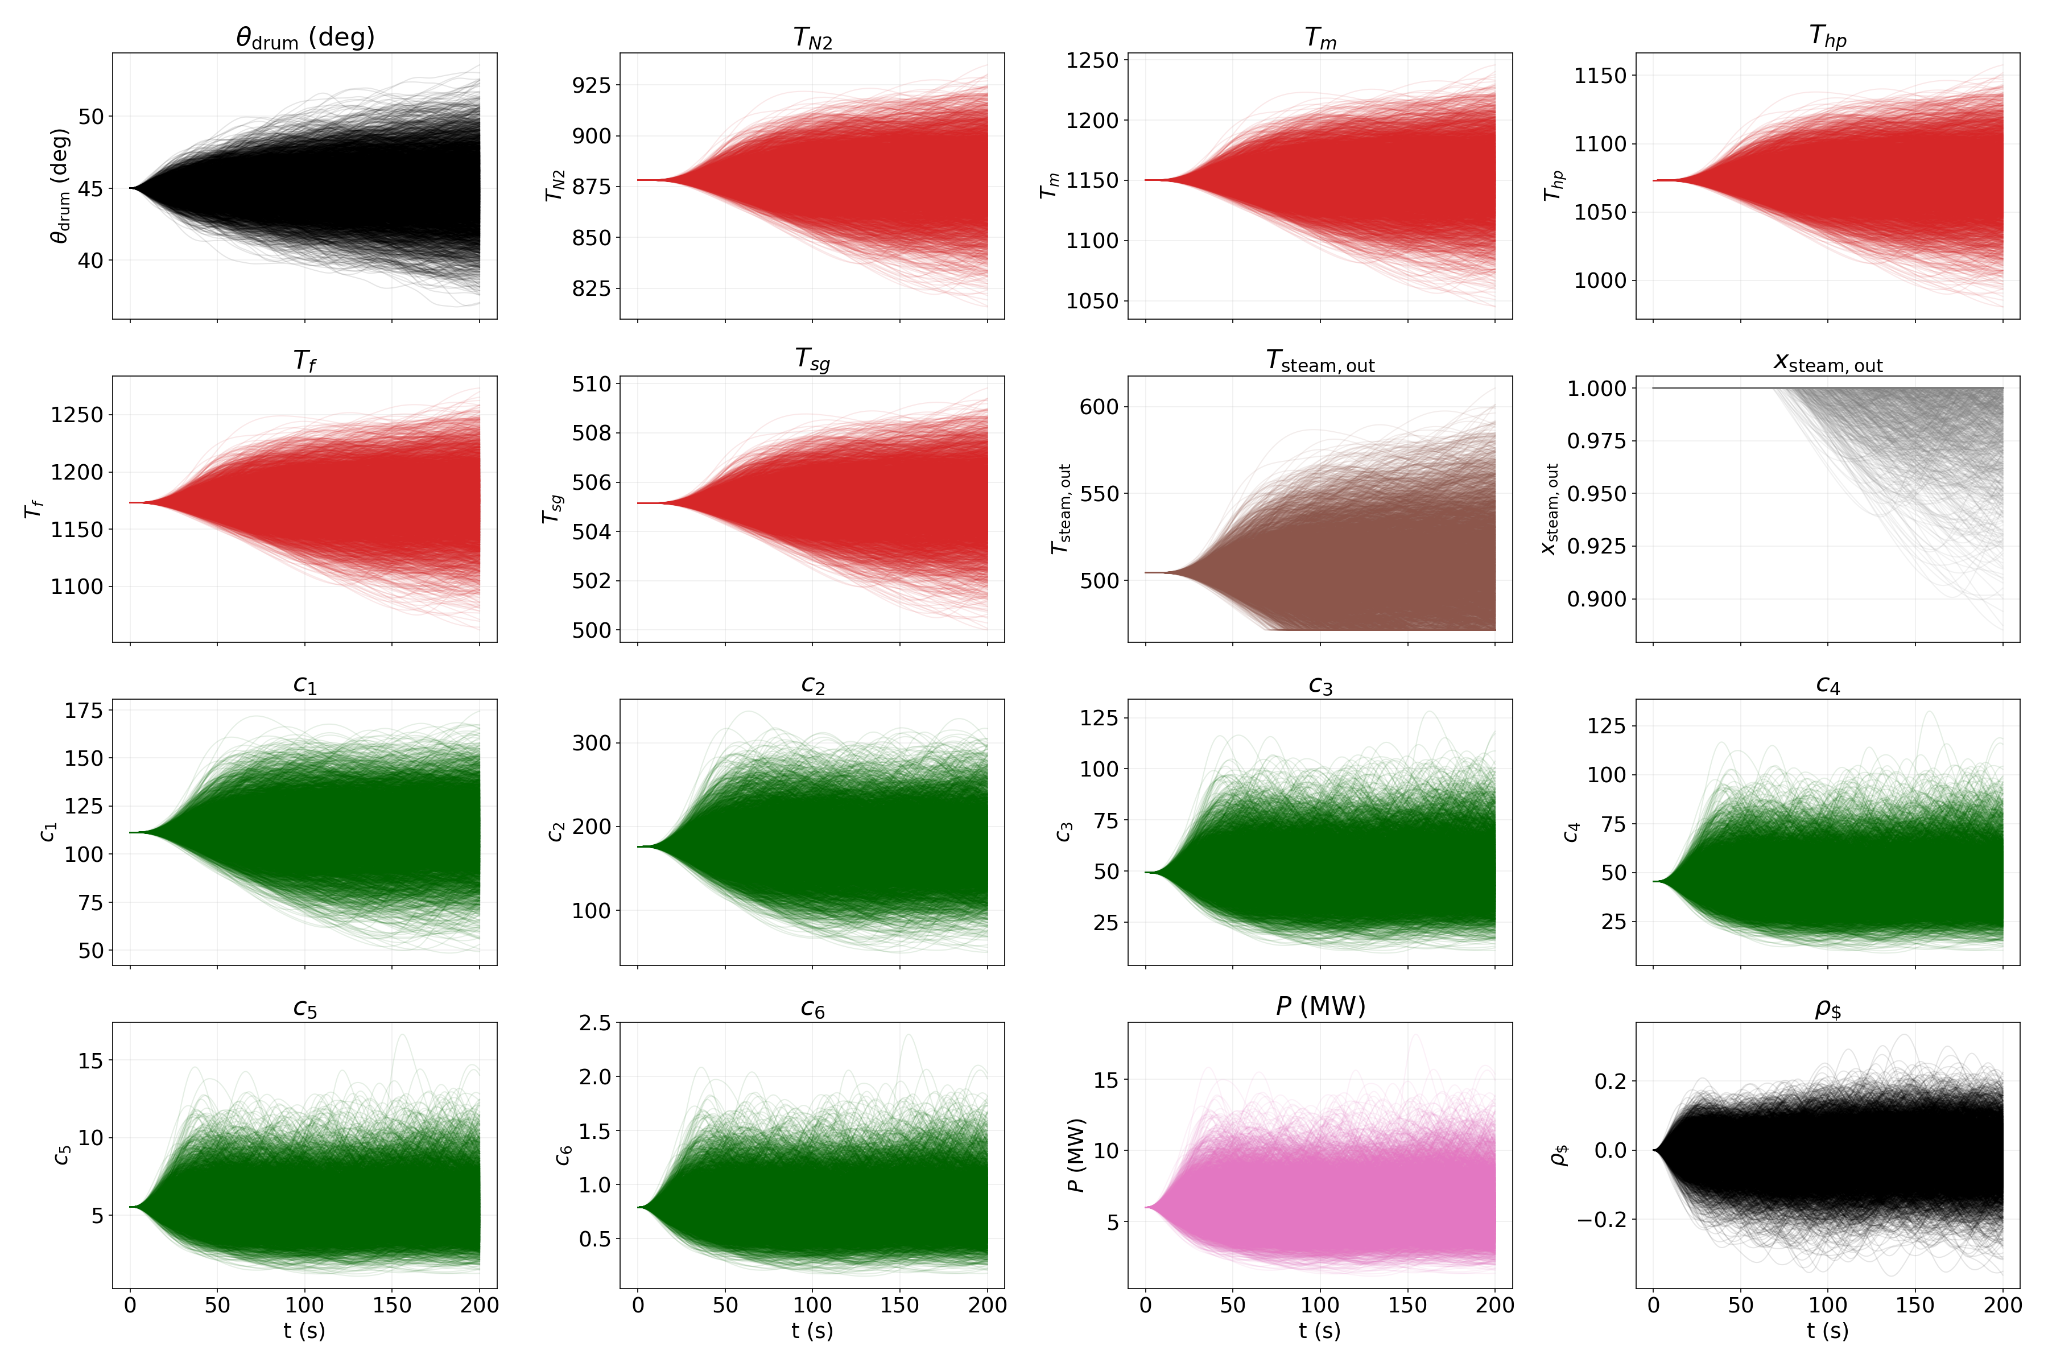
\includegraphics[width=\textwidth]{docs/paper/assets/timeseries_batch_0003_ALL_PROFILES.png}
\caption{Illustration of generated stochastic transients in batch 0003 on the 0--200-s grid. The 4$\times$4 layout shows (row 1) prescribed drum angle, $T_{N2}$, $T_m$, $T_{hp}$; (row 2) $T_f$, $T_{sg}$, $T_{\mathrm{steam,out}}$, steam quality; (row 3) $c_1$--$c_4$; and (row 4) $c_5$, $c_6$, physical power $P$ (MW), and $\rho_{\$}$. The first panel is an input, not one of the 15 predicted outputs. These are simulator responses; the image alone does not independently establish batch count or train-split membership.}
\label{fig:mace:dataset}
\end{figure*}

\subsection{Calibration distributions and operation-informed comparison}
\label{sec:methods:transfer}

We assess the frozen ensemble in two related settings. The original stochastic evaluation distribution provides the reference check of recursive prediction and uncertainty calibration under the original control generator, subject to reconciling its archived recurrence. The second setting deliberately changes the control-trajectory distribution to a prespecified operation-informed mixture. It separates failure of a transferred interval calibration from deterioration in mean forecasting: the same model forecasts are evaluated with alternative quantiles, rather than retraining after observing operational trajectories.

The retained operation-informed population contains four equally probable control families, labeled B, C, D, and F as study-specific identifiers. Family B executes an upward constant-speed maneuver followed by a hold; C makes three upward increments with intermediate holds; D advances and returns to $45^\circ$; and F makes successive positive and negative excursions before returning to the baseline. Parameters for start time, target angle, rate or duration are sampled independently within each family, then maneuver times are rounded to the 0.4-s response grid. Realized velocities are obtained from the rounded endpoints, not simply identified with the requested rate draws. The allowed local-study angles lie within $44.25^\circ$--$48.75^\circ$; the implemented recipe rejects overlaps, out-of-domain moves, and rates outside its local admissibility checks. The piecewise-linear control has finite velocity during motion and idealized velocity jumps at maneuver corners; no finite-acceleration actuator dynamics are assessed. The specific family probabilities and maneuver ranges are experimental design choices rather than empirically measured operational frequencies. The calibration and evaluation sets contain 1,000 and 2,000 independent trajectories, respectively, generated using separate random-number streams with seed 20261010.

\begin{table*}[t]
\centering\small
\caption{Prespecified operation-informed control families. Times are seconds, angles are degrees, and speeds are degrees per second. Values are nominal parameter-draw intervals before rounding schedule times to the 0.4-s grid; realized speeds are calculated from the rounded controls. These ranges are study choices, not measured maneuver frequencies.}
\label{tab:mace:families}
\begin{tabular}{@{}lp{0.21\textwidth}p{0.23\textwidth}p{0.36\textwidth}@{}}
\toprule
Family & Maneuver pattern & Start-time ranges (s) & Amplitude, duration, and rate design\\
\midrule
B & One upward move and hold & 24--56 & Rise 1--3$^\circ$; requested speed 0.05--0.15$^\circ$/s.\\
C & Three upward moves with holds & 24--36; 74--86; 130--142 & Each increment 0.5--1.25$^\circ$; requested speed 0.08--0.16$^\circ$/s.\\
D & Upward move, hold, return & 20--32; 116--124 & Upward rise 2--3$^\circ$; each duration 40--60 s before grid rounding.\\
F & Above baseline, below baseline, return & 32--48; 84--100; 140--152 & Intermediate levels 45.25--45.75$^\circ$ and 44.25--44.75$^\circ$; requested speed 0.04--0.12$^\circ$/s.\\
\bottomrule
\end{tabular}
\end{table*}

On the \emph{same} operation-informed evaluation forecasts, we compare (i) quantiles from the original stochastic calibration trajectories, regenerated with the corrected feedback convention, and (ii) quantiles from an independent operation-informed calibration set sampled from the same B/C/D/F mixture. The former is a \emph{distribution-transfer diagnostic}: the calibration and evaluation trajectory samples are not assumed exchangeable and nominal split-conformal coverage is not asserted. In the latter comparison, the common mixture supports the pooled marginal event under trajectory-level exchangeability; it does not guarantee nominal coverage within every maneuver family. The ten model checkpoints, training scaler, initial history convention, common floor, prescribed operational controls, ensemble means, and ensemble spreads remain fixed between arms. Recalibration changes only the empirical quantiles and interval endpoints, not the mean forecast. Absolute-error conformal baselines are recalibrated separately in each matching arm.

The maneuver phase is identified from the control schedule before examining forecast errors. Motion is the half-open interval $[t_{\mathrm{start}},t_{\mathrm{end}})$ for each move. Early settling covers the following 20~s, excluding any overlap with a new motion interval; initial hold precedes the first move, and late hold includes other stationary periods. Phase statistics do not use separately phase-calibrated thresholds. This permits interpretation of forecast behavior during movement and thermal relaxation without reassigning the population-level coverage guarantee to each phase. Figure~\ref{fig:mace:design} summarizes the frozen-model calibration comparison and the prescribed families.

\begin{figure*}[t]
\centering
% Top panel for Figure 6; bottom controls are produced by the manifest-driven renderer.
\resizebox{\textwidth}{!}{%
\begin{tikzpicture}[>=Latex,font=\sffamily\scriptsize,
 n/.style={draw=black!70,rounded corners=2pt,fill=blue!3,align=center,minimum height=.7cm,inner sep=4pt},
 ar/.style={-{Latex[length=2.2mm]},line width=.65pt,draw=black!70}]
 \node[anchor=west,font=\bfseries\small] at (-.1,4.02) {(a) Same frozen predictor; two calibration distributions};
 \node[n,minimum width=2.65cm] (train) at (1.5,2.95) {Stochastic training 5,000\\validation 1,000};
 \node[n,minimum width=3.2cm,fill=blue!9] (freeze) at (5.3,2.95) {Ten frozen LSTM members\\training scaler; common floor};
 \node[n,minimum width=3.05cm] (calo) at (9.5,3.45) {Original stochastic\\calibration 1,000};
 \node[n,minimum width=3.05cm] (caln) at (9.5,2.28) {Operation-informed\\calibration 1,000};
 \node[n,minimum width=3.6cm,fill=orange!7] (test) at (14.15,2.95) {Same operation-informed evaluation\\2,000 trajectories; frozen forecasts};
 \draw[ar] (train)--(freeze);
 \draw[ar] (freeze)--(calo.west);
 \draw[ar] (freeze)--(caln.west);
 \draw[ar] (calo)--node[above,sloped,font=\tiny,fill=white] {Transferred quantiles} (test);
 \draw[ar] (caln)--node[below,sloped,font=\tiny,fill=white] {Recalibrated quantiles} (test);
 \draw[ar] (freeze) to[out=15,in=170] node[above,font=\tiny,fill=white,pos=.53] {Same mean and spread} (test);
 \node[n,minimum width=2.65cm,fill=black!2] (origtest) at (1.55,1.25) {Stochastic evaluation 2,000\\original-distribution arm};
 \draw[ar,dashed] (freeze.south west) to[out=-130,in=80] (origtest.north east);
 \draw[ar,dashed] (calo.south west) to[out=200,in=10] (origtest.east);
 \node[anchor=west,font=\scriptsize] at (4.1,1.3) {Original $\rightarrow$ operation-informed: distribution-transfer diagnostic};
 \node[anchor=west,font=\scriptsize] at (4.1,.80) {Operation-informed calibration/evaluation: independent draws from one B/C/D/F mixture};
 \node[anchor=west,font=\scriptsize] at (4.1,.30) {Quantiles recalculated for Horizon, per-output Trajectory, and joint Trajectory objectives};
 \node[font=\scriptsize,text=black!75,anchor=west] at (.05,-.26) {Model checkpoints, scaler, control trajectories, forecast mean, and spread are not updated by recalibration.};
\end{tikzpicture}%
}

\par\vspace{2mm}
\includegraphics[width=0.96\textwidth]{outputs/paper/mace_figures/operational_controls/fig06_bcde_operational_controls.pdf}
\caption{Calibration-transfer evaluation with a common frozen predictor. (a) Original stochastic calibration and independent operation-informed calibration produce different interval quantiles for identical operation-informed forecast means and spreads; original-to-operational transfer is a diagnostic, while pooled exchangeability is assumed only within the independently sampled operation-informed mixture. (b--e) Prescribed B/C/D/F control families, showing three lowest-ID evaluation profiles per family when the retained manifest is available. Identical angle/time axes, baseline, and line-style conventions are used; the illustrated controls are selected without forecast-performance information.}
\label{fig:mace:design}
\end{figure*}

\begin{table}[t]
\centering\small
\caption{Evaluated distribution comparisons and what remains fixed. The shared operation-informed evaluation samples prevent a change in the point predictor from being mistaken for recalibration.}
\label{tab:mace:arms}
\begin{tabular}{@{}p{0.27\linewidth}p{0.26\linewidth}p{0.28\linewidth}@{}}
\toprule
Calibration source & Evaluation population & Interpretation\\
\midrule
Stochastic (1,000) & Stochastic (2,000) & Original-distribution conformal comparison, pending corrected-forecast provenance\\
Stochastic (1,000) & Operation-informed (2,000) & Calibration-transfer diagnostic; no ordinary exchangeability claim\\
Operation-informed (1,000) & Operation-informed (same 2,000) & Pooled mixture marginal calibration under independent matched draws\\
\bottomrule
\end{tabular}
\end{table}

\subsection{Evaluation metrics and uncertainty in comparisons}
\label{sec:methods:metrics}

Forecast accuracy is evaluated against the simulator's native physical output values using per-output mean absolute error (MAE) and root-mean-square error (RMSE). For equal-output aggregate comparisons, per-output absolute errors are divided by the saved training output spans $b_j^Y$ before averaging. Aggregate normalized MAE is the equal-output mean of normalized MAEs, while aggregate normalized RMSE is the square root of the equal-output mean normalized mean-squared errors; it is not the arithmetic mean of per-output RMSEs. Recursive accuracy is reported separately from calibration and is further partitioned by family and maneuver phase.

Let $A_{i,h,j}=\mathbf{1}\{L_{i,h,j}\leq\widetilde y^{\,Y}_{i,h,j}\leq U_{i,h,j}\}$ denote inclusive coverage by scaled-space endpoints. Four distinct empirical quantities are recorded: pointwise $(h,j)$ coverage, $N_{\rm eval}^{-1}\sum_i A_{i,h,j}$; per-output trajectory coverage, $N_{\rm eval}^{-1}\sum_i\prod_h A_{i,h,j}$; Horizon complete multivariate coverage, $N_{\rm eval}^{-1}\sum_i\prod_j A_{i,h,j}$ at fixed $h$; and Trajectory complete multivariate coverage, $N_{\rm eval}^{-1}\sum_i\prod_{h,j}A_{i,h,j}$. A mean across output-specific trajectory coverages is not the complete multivariate event. Phase-restricted trajectory coverage applies the same products only to supported phase times and excludes trajectories without phase support; it is reported as a diagnostic rather than an additional guaranteed event.

Interval efficiency is measured by full width $W=U-L$, in scaled units for cross-output aggregates and after multiplication by $b_j^Y$ for output-specific physical widths. The paired MACE-to-absolute-CP width ratio is computed from pooled mean widths, $\overline W_{\rm MACE}/\overline W_{\rm abs}$, with proportional reduction $1-\overline W_{\rm MACE}/\overline W_{\rm abs}$. As a complementary measure of sharpness and miss magnitude, we use the interval score~\cite{gneiting2007scoring},
\begin{equation}
 {\rm IS}_{\alpha}(L,U;y)
 =(U-L)+\frac{2}{\alpha}(L-y)\mathbf{1}\{y<L\}
        +\frac{2}{\alpha}(y-U)\mathbf{1}\{y>U\}.
 \label{eq:mace:intervalscore}
\end{equation}
Lower scores are preferable. For the trajectory procedures this is a \emph{point-averaged endpoint diagnostic}, not a proper joint-trajectory scoring rule and not an alternative to measuring the appropriate simultaneous coverage event.

Pointwise accuracy, width, and interval scores pool sums and counts across supported time points, preserving the actual differences in dwell time. Across variables, scaled aggregate summaries use equal output weights. For trajectory coverage, each supported trajectory contributes one success or failure, regardless of phase duration. We report support counts and distinguish all-time, motion, early-settling, late-hold, and initial-hold results so that long stationary periods cannot conceal missed transients.

Uncertainty in comparisons is estimated using 10,000 paired whole-trajectory nonparametric bootstrap replicates with seed 20261011. Evaluation trajectory IDs are sampled with replacement, retaining each sample's entire time series, all output variables, family labels, phase masks, and all method/calibration-arm results. The same bootstrap draw is used for every paired difference and width ratio, which is recomputed from replicate mean widths. Two-sided 95\% percentile intervals summarize evaluation-sample variation conditional on the fitted models and calibration sets; they do not account for retraining or repeated recalibration. Family-specific comparisons filter the common draws to that family rather than imposing fixed family counts on every replicate. These intervals do not constitute simultaneous inference over all output--horizon or family--phase comparisons.

For numerical consistency, conformal scores, quantiles, and endpoints are constructed in output-scaled float32 arrays. Coverage is decided inclusively in those same coordinates; endpoints and truth are subsequently promoted to float64 for width and interval-score arithmetic. Physical accuracy retains native simulator truth. Inverse transformations used for presentation do not trigger a second, differently rounded coverage test. The reproducibility record must identify the checkpoint/scaler hashes, partition manifests, recurrence convention, calibration quantiles, and source commits, and must reconcile the original stochastic forecast archive before final results are quoted.
